\documentclass[12pt]{article}
\usepackage[czech]{babel}
\usepackage[utf8]{inputenc}
\usepackage[plainpages=false,pdfpagelabels,unicode]{hyperref}
\usepackage[pdftex]{graphicx}
\usepackage[margin=2cm, includefoot]{geometry}

\begin{document}

\title{Praktikum z fyziky plazmatu \\
Měření rozdělovací funkce energie elektronů pomocí Langmuirovy sondy}
\author{Pavel Ondračka}
\maketitle

\section{Teorie}

\subsection{Druyvensteynova formule}

Z VA charakteristiky Langmuirovy sondy můžeme určit rozdělovací funkce elektronů pomocí Druy\-ven\-steynovy furmule
\begin{equation}
f(e|U_\mathrm{pl}-U_\mathrm{s}|)= \frac{2 \sqrt{2 m_e |U_\mathrm{pl}-U_\mathrm{s}|}}{e^{5/2} A} \frac{\mathrm{d}^2 I_\mathrm{se}}{\mathrm{d}U_\mathrm{s}^2} \mathrm{,}
\end{equation}
kde $U_\mathrm{s}$ je napětí na sondě, $U_\mathrm{pl}$ je potenciál plazmatu, $A$ je plocha sondy a $I_\mathrm{se}$ je sondový elektronový proud). Druhou derivaci lze získat buď přímo derivací elektronového proudu, nevýhodou je vznik šumu vlivem numerické derivace, nebo přiložením slabého střídavého napětí $U_1$ na sondu. Pak platí
\begin{equation}
\Delta I_\mathrm{s} = \frac{U_1^2}{4} \frac{\mathrm{d}^2 I_\mathrm{s}}{\mathrm{d}U_\mathrm{s}^2} \mathrm{,}
\end{equation}
kde $\Delta I_\mathrm{s}$ je změna sondového proudu po zapnutí střídavého napětí.

Z rozdělovací funkce lze spočítat elektronovou koncentraci a střední energii běžným způsobem, jako integrály z rozdělovací funkce
\begin{equation}
n_\mathrm{e} = \int_{-\infty}^{U_\mathrm{pl}} e f(e(U_\mathrm{pl}-U_\mathrm{s})) \mathrm{d}U_\mathrm{s}
\end{equation}
\begin{equation}
<E> =  \frac{1}{n_\mathrm{e}} \int_{-\infty}^{U_\mathrm{pl}} e^2 (U_\mathrm{pl}-U_\mathrm{s}) f(e(U_\mathrm{pl}-U_\mathrm{s}))  \mathrm{d}U_\mathrm{s}
\end{equation}

\subsection{Rozdělovací funkce nabitých částic v plazmatu}
Řešením Boltzmannovy kinetické rovnice pro bezsrážkové, homogenní plazma ve stacionárním stavu bez působení vnějších sil je Maxwellova rozdělovací funkce

\begin{equation}
f_\alpha (E) = 2 n_\alpha \pi ( \pi k T_\alpha)^{-3/2} \sqrt{E}\, \mathrm{exp} (-\frac{E}{2kT_\alpha}) \mathrm{.}
\end{equation}

Maxwellova funkce je ale řešením BKR jen za velmi omezujících předpokladů. Obecně můžeme na dané rozdělení fitovat tzv. Standardní rozdělení 

\begin{equation}
f_\alpha (E) = A \sqrt{E} \, \mathrm{exp} (-\frac{E^\kappa}{\kappa E_\mathrm{p}^\kappa}) \mathrm{,}
\end{equation}

kde A je normovací konstanta, $E_\mathrm{p}$ je nejpravděpodobnější energie částic a $\kappa$ závisí na rozdělení. Pro $\kappa = 1$ se jedná o Maxwellovo rozdělení, pro $\kappa = 2$ se jedná o Druyvesteynovo rozdělení atd. Pomocí fitování volných parametrů $\kappa$ a $E_\mathrm{p}$ lze tedy zjistit typ rozdělení.

\begin{figure}[htbp]
\begin{center}
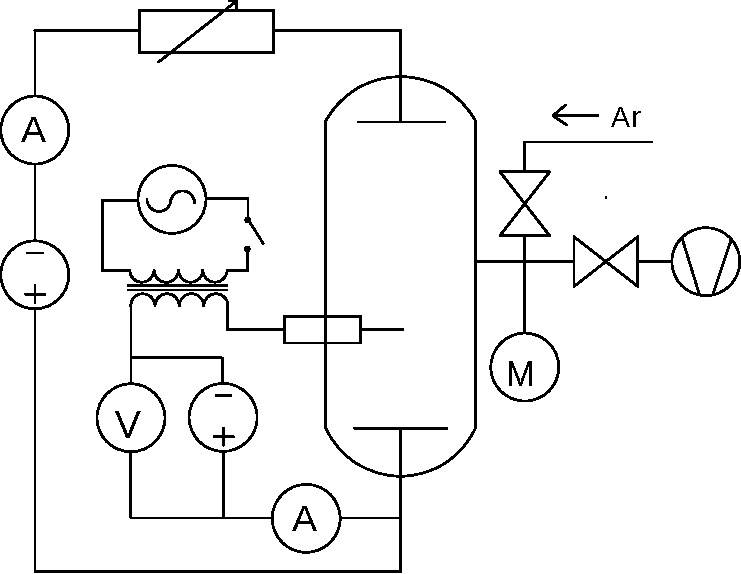
\includegraphics[width=12cm]{schema.pdf}
\caption{Schéma aparatury}
\label{schema}
\end{center}
\end{figure}

\section{Měření}
Pro měření bylo použita jednoduchá rovinná sonda s průměrem asi 2\,mm, střídavé napětí $U_1$ bylo 3,95\,V (bohužel bylo opomenuto změřit a bylo doměřováno až následující týden, proto mohla být skutečná hodnota úplně jiná). Naměřené sondové proudy jsou na obrázku \ref{proud}. Pro metodu numerického určení druhé derivace jsou určené experimentální rozdělovací funkce spolu s fity teoretických rozdělovacích funkcí  na obrázcích \ref{iv32} a \ref{iv40} a výsledky shrnuje tabulka \ref{vysledky}. Pro metodu druhé derivace získané aplikací slabého střídavého napětí jsou určené experimentální rozdělovací funkce spolu s fity teoretických rozdělovacích funkcí  na obrázcích \ref{iv32d} a \ref{iv40d} a výsledky shrnuje tabulka \ref{vysledky2}. Elektronová koncentrace a střední energie byly určeny jen pro metodu numerické derivace, protože u druhé metody rozdělovací funkce nekonvergovala k nule, proto také bylo fitování omezeno jen na oblast kde měla funkce očekávaný tvar.

\begin{figure}[htbp]
\begin{center}
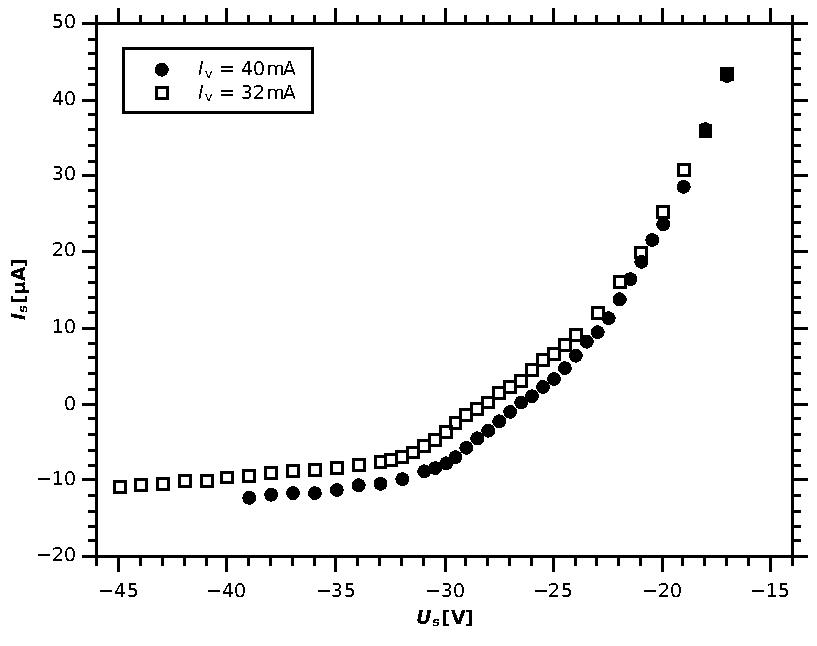
\includegraphics[width=12cm]{Graph1.pdf}
\caption{Naměřené sondové proudy}
\label{proud}
\end{center}
\end{figure}

\begin{figure}[htbp]
\begin{center}
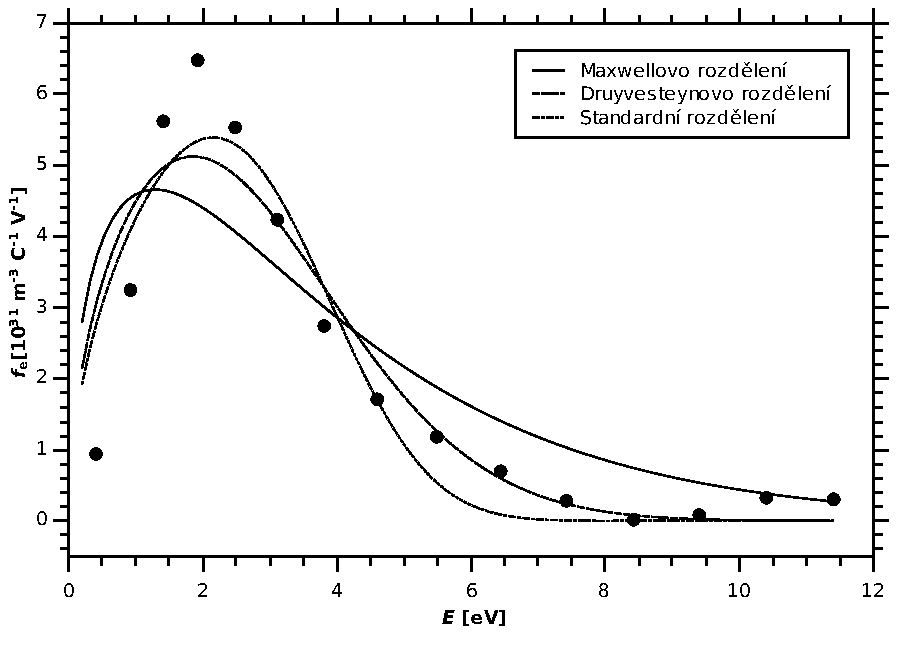
\includegraphics[width=12cm]{iv32dist.pdf}
\caption{Elektronová experimentální rozdělovací funkce (druhá derivace získána numericky) pro výbojový proud $I_\mathrm{v} = 32$\,mA a fity některých běžných rozdělovacích funkcí}
\label{iv32}
\end{center}
\end{figure}

\begin{figure}[htbp]
\begin{center}
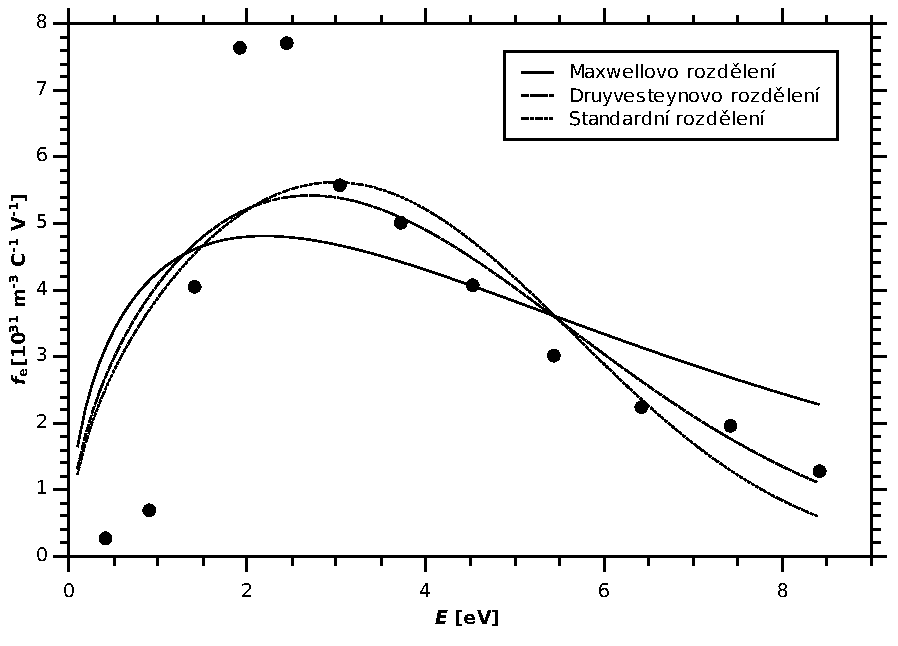
\includegraphics[width=12cm]{Iv40dist.pdf}
\caption{Elektronová experimentální rozdělovací funkce (druhá derivace získána numericky) pro výbojový proud $I_\mathrm{v} = 40$\,mA a fity některých běžných rozdělovacích funkcí}
\label{iv40}
\end{center}
\end{figure}

\begin{figure}[htbp]
\begin{center}
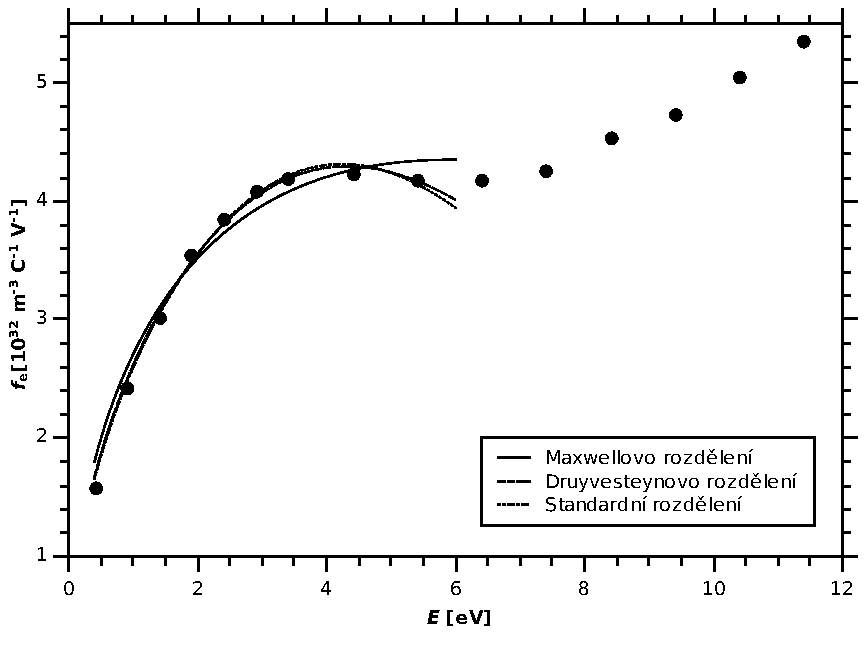
\includegraphics[width=12cm]{iv32druv-img.pdf}
\caption{Elektronová experimentální rozdělovací funkce (druhá derivace získána aplikací střídavého napětí) pro výbojový proud $I_\mathrm{v} = 32$\,mA a fity některých běžných rozdělovacích funkcí}
\label{iv32d}
\end{center}
\end{figure}

\begin{figure}[htbp]
\begin{center}
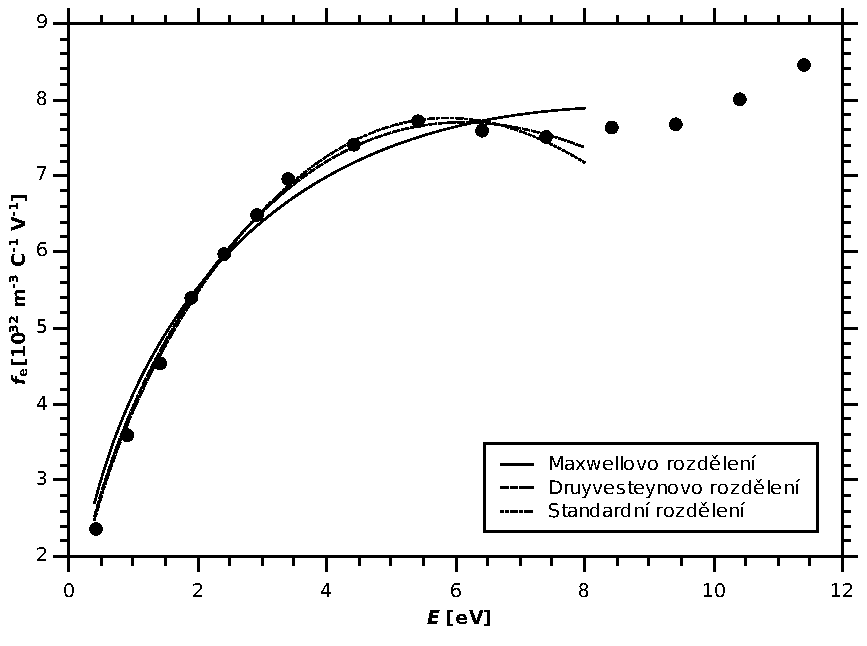
\includegraphics[width=12cm]{iv40druv-img.pdf}
\caption{Elektronová experimentální rozdělovací funkce (druhá derivace získána aplikací střídavého napětí) pro výbojový proud $I_\mathrm{v} = 40$\,mA a fity některých běžných rozdělovacích funkcí}
\label{iv40d}
\end{center}
\end{figure}

\begin{table}[htbp]
\begin{center}
\begin{tabular}{|c|c|c|c|c|c|c|c|}
\hline
$I_\mathrm{v}$[mA] & $U_\mathrm{pl}$[V] & $S_\mathrm{Max}[10^{62}]$ & $S_\mathrm{Druy}[10^{62}]$ & $S_\mathrm{Stan}[10^{62}]$ & $\kappa$ & $n_\mathrm{e}$ [10$^{13}$ m$^{-3}$] & $<E>$[eV] \\ \hline
32 & -29,6 & 19,5 & 8,96 & 7,17 & 3,1$\pm$0,9 & 3,28 & 3,82 \\ \hline
40 & -27,6 & 40,7 & 28,7 & 27,3 & 2,7$\pm$1,5 & 4,67 & 3,05 \\ \hline
\end{tabular}
\caption{Výsledky měření (druhá derivace získána numericky), $S_\mathrm{Max}$, $S_\mathrm{Druy}$ a $S_\mathrm{Stan}$ jsou příslušné reziduální sumy čtverců jednotlivých fitů.}
\label{vysledky}
\end{center}
\end{table}

\begin{table}[htbp]
\begin{center}
\begin{tabular}{|c|c|c|c|c|c|c|c|}
\hline
$I_\mathrm{v}$[mA] & $U_\mathrm{pl}$[V] & $S_\mathrm{Max}[10^{63}]$ & $S_\mathrm{Druy}[10^{62}]$ & $S_\mathrm{Stan}[10^{62}]$ & $\kappa$\\ \hline
32 & -29,6 & 1,69 & 2,37 & 2,37 & 2,24$\pm$0,29 \\ \hline
40 & -27,6 & 6,53 & 11,5 & 7,31 & 2,47$\pm$0,26 \\ \hline
\end{tabular}
\caption{Výsledky měření (druhá derivace získána aplikací střídavého napětí), $S_\mathrm{Max}$, $S_\mathrm{Druy}$ a $S_\mathrm{Stan}$ jsou příslušné reziduální sumy čtverců jednotlivých fitů.}
\label{vysledky2}
\end{center}
\end{table}


\section{Závěr}
Měření proběhlo úspěšně, podařilo se naměřit VA charakteristiku jednoduché rovinné sondy a z~ní určit elektronovou rozdělovací funkci pomocí Druyvesteynovy formule. Ukázalo se, že funkce nejsou maxwellovské, ale spíše se podobají rozdělovacím funkcím Druyvesteynovým, což by odpovídalo podmínkám (homogenní el. pole), i když fitováním Standardního rozdělení se ukázalo, že $\kappa$ je přibližně 2--3, tj. někde mezi Druyvesteinovou ($\kappa = 2$) a Davidovou ($\kappa=4$) rozdělovací funkcí. Pro metodu numerické derivace bohužel experimentální funkce na fit moc nesedí pro nízké energie, kde naměřená rozdělovací funkce roste moc pomalu, naopak maximum  experimentální funkce je výrazně výš než bychom očekávali. Pro metodu střídavého napětí sedí fity dobře pro nízké energie, ale pro vysoké energie rozdělovací funkce divergují. Hodnoty rozdělovací funkce jsou pro tuto metodu asi o řád vyšší, to je pravděpodobně způsobeno špatnou hodnotou $U_1$, která byla doměřována později a také tím, že vztah platí jen pro malá $U_1$, což nebylo splněno. Další problémy, které se vyskytly během měření, byly třeba že  plazmový potenciál vyšel pod plovoucím potenciálem, což je v rozporu s teorií a při změně napětí na sondě někdy trvalo delší dobu (řádově desítky sekund) než se ustálil sondový proud. Toto bylo pravděpodobně způsobeno nějakými změnami na sondě (zahřívání), protože plazma se při podmínkách použitých v experimentu dostává do rovnováhy mnohem rychleji. Naměřené elektronové koncentrace se jsou asi o 50\,\% nižší než koncentrace změřené v dřívějším praktiku na stejné aparatuře se stejnou sondou při velmi podobných podmínkách. Dle mého názoru je to způsobeno velkou chybou numerické integrace při malém počtu naměřených bodů. Určování průměru sondy odhadem přesnosti měření také nepřidalo. 

\end{document}
